% 原文 pp.33--39、2.4節導入と2.4.1--2.4.2。
\subsectionlink{密度行列の概念と解釈}
密度行列、とりわけ、いわゆる縮約密度行列は、デコヒーレンスの形式的記述において重要な役割を果たす。この主な理由は、系と環境の量子もつれによって、系に個別の量子状態ベクトルを割り当てることが不可能になり（前の2.3節）、したがって通常、関心のある系を、そのような純粋量子状態によって記述できないことにある。後に見るように、縮約密度行列は、その場合に、系の測定統計を表す洗練された方法を与える。以下では、純粋状態、混合状態、および縮約密度行列のさまざまな側面を、時間をかけて論じる。

% 原文 p.34
\hypertarget{srcpage:34}{}\label{srcpage:34}
\subsubsectionlink{純粋状態の密度行列とトレース演算}
なじみ深い量子状態ベクトルの概念から始めよう。上で説明したように、量子状態ベクトル$\lvert\psi\rangle$は、物理系の状態についての最大の知識を包含する。そのような純粋状態$\lvert\psi\rangle$に対応する密度演算子$\hat\rho$を、
\begin{equation}\hat\rho\equiv\lvert\psi\rangle\langle\psi\rvert\tag{2.11}\end{equation}
と定義することもできる。これは単に、状態$\lvert\psi\rangle$への射影演算子である。本書では、密度演算子$\hat\rho$に対して、密度行列という語も区別せず用いる。厳密に言えば、密度行列とは、ある特定の基底における密度演算子の行列表現を指すが、演算子$\hat\rho$に「密度行列」を用いることは文献で十分定着しているので、この広く受け入れられた用語法に従う。密度演算子の行列表現を明示的に指したい場合には、$\hat\rho$から演算子を示す帽子を外すことにより、区別を明らかにする。すなわち、そのような実際の密度行列を$\rho$と書く。

$\lvert\psi\rangle$を、基底状態$\lvert\psi_i\rangle$の重ね合わせとして
\begin{equation}\lvert\psi\rangle=\sum_i c_i\lvert\psi_i\rangle\tag{2.12}\end{equation}
と表すと、この基底$\{\lvert\psi_i\rangle\}$で書いた対応する密度行列は、
\begin{equation}\hat\rho=\lvert\psi\rangle\langle\psi\rvert=\sum_{ij}c_ic_j^*\lvert\psi_i\rangle\langle\psi_j\rvert\tag{2.13}\end{equation}
となる。右辺の$i\ne j$の項は、異なる成分$\lvert\psi_i\rangle$間の量子コヒーレンスを表す。したがって、通常は干渉項、あるいは非対角項と呼ばれる。これらは$\{\lvert\psi_i\rangle\}$基底での$\hat\rho$の行列表現の非対角要素に対応するからである。

ただし、そのような干渉項は、常に特定の基底$\{\lvert\psi_i\rangle\}$に関して理解すべきものであることを忘れてはいけない。つまり、コヒーレンスや干渉は、ある特定の成分$\lvert\psi_i\rangle$間に存在する。密度行列を対角化する基底は必ず存在し、その基底には干渉項がない。したがって、干渉（コヒーレンス）を系の「量子性」と結び付けることによって、ある基底で書いた密度行列に干渉項がないなら、系が「量子的性質を持たない」あるいは「古典的に振る舞う」と必ず言える、という誤った結論に至ってはならない。密度行列がそのような対角形になる基底は、経験上なじみのある確定した量と、まったく対応しないかもしれない（2.15.1節も参照）。異なる基底で表すと、一般に干渉項は再び現れ、それらの基底状態間の量子コヒーレンスが存続していることを示す。

% 原文 p.35
\hypertarget{srcpage:35}{}\label{srcpage:35}
次に「$\operatorname{Tr}$」と書くトレース演算を導入しよう。この演算は常に、何らかの演算子$\hat A$に作用し、次のように実行する。系のHilbert空間の正規直交基底$\{\lvert\phi_i\rangle\}$を選び、
\begin{equation}\operatorname{Tr}(\hat A)\equiv\sum_i\langle\phi_i\rvert\hat A\lvert\phi_i\rangle\tag{2.14}\end{equation}
を計算する。この演算が線形であること、
\begin{equation}\operatorname{Tr}(\hat A+\hat B)=\operatorname{Tr}(\hat A)+\operatorname{Tr}(\hat B)\tag{2.15}\end{equation}
および正規直交基底$\{\lvert\phi_i\rangle\}$の具体的な選び方に依存しないことは、容易に示せる。したがってトレースを計算するには、任意の正規直交基底ベクトルの組を用いてよい。

なぜトレース演算を導入するのだろうか。これに答えるため、純粋状態の密度行列(2.11)と、系で測定する何らかの観測可能量を表すHermite演算子$\hat O$の積からなる、演算子$\hat A=\hat\rho\hat O$を考えよう。$\hat\rho\hat O$のトレース(2.14)を求めるための正規直交基底として、$\hat O$の固有状態$\lvert o_i\rangle$を選び、対応する固有値を$o_i$とする（ここでは離散スペクトルを仮定する）。すると、
\begin{equation}\operatorname{Tr}(\hat\rho\hat O)=\sum_i\langle o_i\rvert(\lvert\psi\rangle\langle\psi\rvert)\hat O\lvert o_i\rangle=\sum_i o_i\lvert\langle o_i\vert\psi\rangle\rvert^2\tag{2.16}\end{equation}
を得る。しかし$\lvert\langle o_i\vert\psi\rangle\rvert^2$は、$\hat O$で表される測定で結果$o_i$が得られるBorn確率にすぎない\footnote{Born則\cite{ref019}は次のように述べられる。系が純粋状態$\lvert\psi\rangle$で記述されるとし、固有状態$\lvert o_i\rangle$と対応する固有値$o_i$を持つHermite演算子$\hat O$で表される観測可能量を、系に対して測定するとする（ここでも$\hat O$の離散スペクトルを仮定する）。すると、(i) 状態$\lvert o_i\rangle$と対応する固有値$o_i$だけが、測定の可能な結果である。(ii) 測定後に状態$\lvert o_i\rangle$に系を見いだす確率、別の言い方をすれば値$o_i$を測定する確率は、$\lvert\langle o_i\vert\psi\rangle\rvert^2$で与えられる。主張(i)は本質的に量子力学の収縮公準であるため、しばしばBorn則から分離され、Born則の内容は、確率の実際の値を計算する処方(ii)だけとされる。}。したがって$\operatorname{Tr}(\hat\rho\hat O)$は、この測定のすべての可能な結果$o_i$を、対応するBorn確率で重み付けした平均を表す。これはまさに、観測可能量$\hat O$の期待値$\langle\hat O\rangle$の定義である。演算子$\hat\rho\hat O$のトレースという数学的手順と、測定の期待値という物理的概念のこの結び付きは、トレース則として知られている\footnote{もちろんトレース則は、$\langle\hat O\rangle=\langle\psi\rvert\hat O\lvert\psi\rangle$による純粋状態の期待値の計算と完全に同値である。系の状態$\lvert\psi\rangle$を含む正規直交基底状態の組を用いてトレース(2.16)を計算すれば、すぐに確認できる。}。
% 原文 p.36
\hypertarget{srcpage:36}{}\label{srcpage:36}
\begin{equation}\langle\hat O\rangle=\operatorname{Tr}(\hat\rho\hat O).\tag{2.17}\end{equation}
$\hat O=\hat I$と選べば、予想どおり
\begin{equation}\operatorname{Tr}\hat\rho=1\tag{2.18}\end{equation}
を得る。これは単に、純粋状態が規格化されていること、すなわち$\lvert\langle\psi\vert\psi\rangle\rvert^2=1$を反映する。先に進む前に、トレースの概念と解釈が、根本的にBorn則に依拠していることを、再び強調しておく。この点の重要性は後に明らかになる。

\subsubsectionlink{混合状態の密度行列}
ここまで、密度行列を使って系の状態を記述しても、実際には何の利点も得られていない。系が完全に既知の量子状態にあるなら、純粋量子状態$\lvert\psi\rangle$による記述と、対応する純粋状態の密度行列(2.11)による記述は、形式的にも物理的にも完全に同値である。しかし、系を混合状態によって記述することもできる。混合状態は、系の状態について情報が不十分であることを表す。すなわち、系は測定前に、互いに直交している必要のない純粋状態$\lvert\psi_i\rangle$のいずれかにあるが、観測者にはどれかが分からない。そのため、各状態$\lvert\psi_i\rangle$に確率$p_i\ge0$を帰属させることしかできない\footnote{簡単のため、ここでは有限次元Hilbert空間の場合を考える。無限次元への一般化はかなり直接的である（たとえば文献\cite{ref058}を参照）。}。

そのような状況は、量子状態の準備に用いる物理的手順が、確率的要素を含む場合に典型的に生じる。ただし、その確率は既知である。たとえば準備装置が、二つの可能な状態$\lvert\psi_1\rangle$、$\lvert\psi_2\rangle$のいずれかを準備できるとする（図2.3）。具体的にどの状態を準備するかは、未知の量子状態にあるスピン$1/2$粒子のスピン測定によって決まり、この測定では「上向き」と「下向き」が等しい確率で得られる（たとえば2.2.2節で述べたStern--Gerlach装置を用いて実現できる）。その測定結果に応じ、装置は、関心のある系を、完全に決定論的に、$\lvert\psi_1\rangle$または$\lvert\psi_2\rangle$の状態に準備する。しかし観測者はスピン測定の結果を調べない。そのため、$\lvert\psi_1\rangle$か$\lvert\psi_2\rangle$の一方が準備されたことだけが分かり、二つのうちどちらかは分からない。もちろん、ここでは準備手順の確率的性格を意図的に導入しているため、やや人為的な例である。しかし、状態準備に使う物理的装置に確率的要素が内在する、別のより現実的な状況を想像するのは容易である。たとえば装置が不完全なため、可能な純粋状態のある範囲を生み出す場合がある。

% 原文 p.37
\hypertarget{srcpage:37}{}\label{srcpage:37}
\begin{figure}[htbp]\centering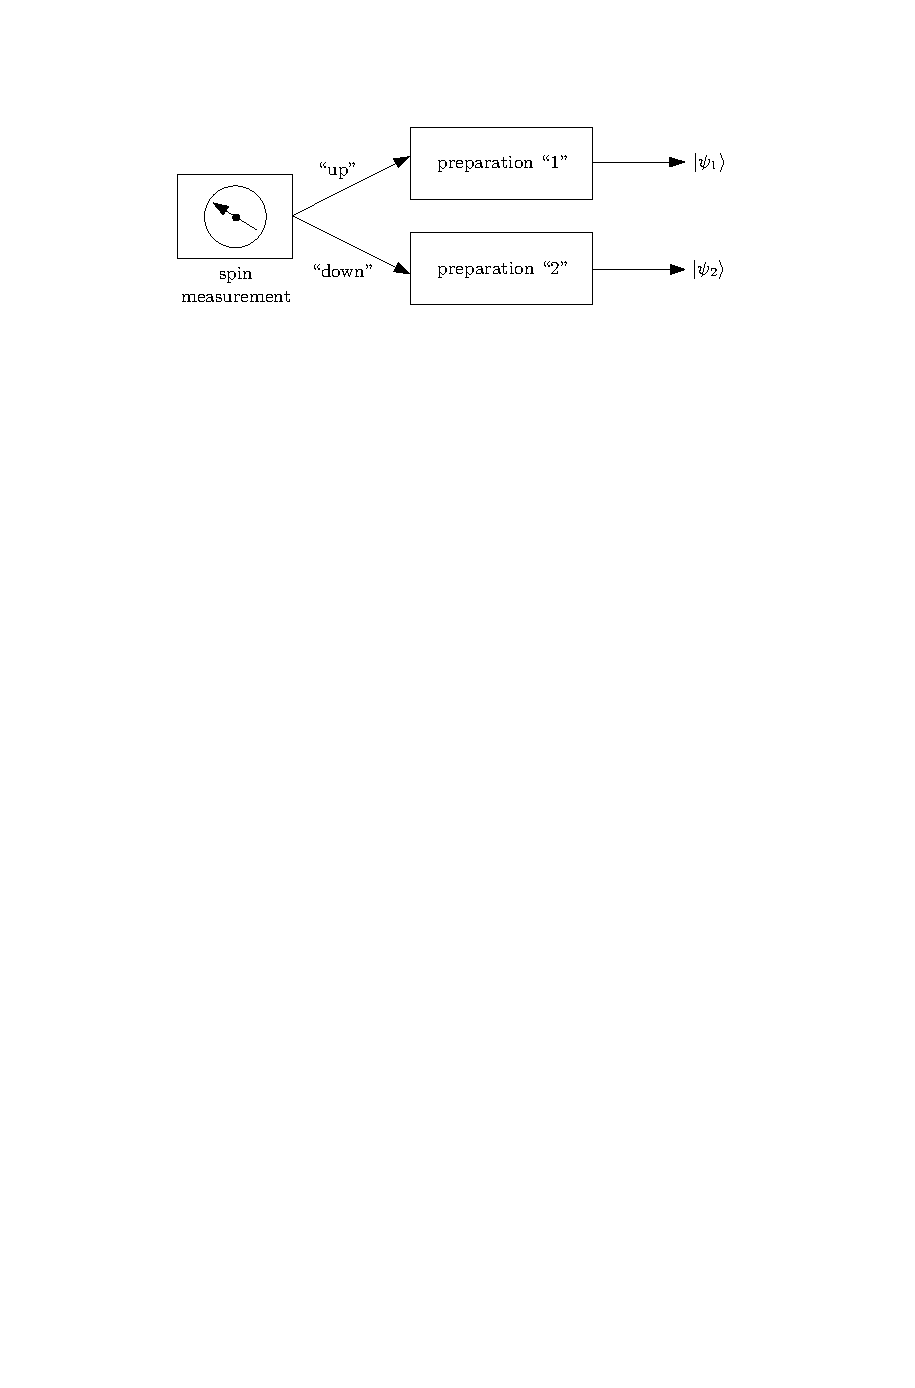
\includegraphics[width=.9\linewidth]{figures/ch02_fig03.pdf}\caption{確率的な状態準備手順の例。スピン$1/2$粒子のスピン測定の結果に応じて、装置は、ある系を量子状態$\lvert\psi_1\rangle$または$\lvert\psi_2\rangle$に準備する。具体的なスピン測定結果を知らない観測者は、状態$\lvert\psi_1\rangle$と$\lvert\psi_2\rangle$に、等しい古典的な確率を割り当てる。この主観的な無知を表すために、準備された系を、混合状態の密度行列$\hat\rho=\frac12\lvert\psi_1\rangle\langle\psi_1\rvert+\frac12\lvert\psi_2\rangle\langle\psi_2\rvert$で記述する。}\end{figure}

確率的要素の物理的な起源が何であれ、混合状態、すなわち確率$p_i$を伴う可能な純粋状態$\lvert\psi_i\rangle$の集合は、古典的な集団を表す。これは、確率の起源が純粋に古典的であることを意味する。これらの確率は、系の量子状態についての観測者の主観的無知を表すにすぎない。物理的には、系は実際に、純粋で、したがって完全に既知の状態に準備されている。ただし観測者には知られていない。原理上、状態準備の手順の各段階をすべて追跡、あるいは遡及すれば、各実行でどの純粋状態$\lvert\psi_i\rangle$が生成されたかを、必ず決められる。確率$p_i$は、準備手順の細かい詳細を調べないという私たちの実際的な選択を表すだけであり、これらの確率には根本的なものはない。したがって、たとえば気体中の個々の分子の決定論的経路を、原理上は追跡できても実際にはできない古典統計力学での「粗視化」と同じ方法に対応するだけである。

% 原文 p.38
\hypertarget{srcpage:38}{}\label{srcpage:38}
混合状態で記述される系について行った測定の統計を、観測者はどのように記述するだろうか。もはや系に純粋量子状態$\lvert\psi\rangle$を割り当てられないので、純粋状態の密度行列$\hat\rho=\lvert\psi\rangle\langle\psi\rvert$を用いた、通常の規則$\langle\hat O\rangle=\langle\psi\rvert\hat O\lvert\psi\rangle$、または$\langle\hat O\rangle=\operatorname{Tr}(\hat\rho\hat O)$［式(2.17)］により、観測可能量$\hat O$の期待値を計算できないことは明らかである。しかしこれらの規則は、準備された系の純粋状態を観測者が知らないことから生じる古典的な確率概念と、量子状態が測定される観測可能量の固有状態へ確率的に「収縮」することから生じる、量子力学固有の確率を組み合わせることで、容易に一般化できる。直観的な考えは、混合状態に含まれる可能な各純粋状態$\lvert\psi_i\rangle$での期待値$\langle\psi_i\rvert\hat O\lvert\psi_i\rangle$を、その状態の古典的確率$p_i$で重み付けし、集団全体について結果を足し合わせるだけである。すなわち、
\begin{equation}\langle\hat O\rangle=\sum_i p_i\langle\psi_i\rvert\hat O\lvert\psi_i\rangle.\tag{2.19}\end{equation}
この式には、まだ別々の二つの統計的要素、すなわち古典的確率$p_i$と、各純粋状態$\lvert\psi_i\rangle$での量子期待値$\langle\psi_i\rvert\hat O\lvert\psi_i\rangle$が含まれる。この両方を包含し、系のすべての統計的性質を完全に符号化する、混合状態の密度行列を導入できる。それは
\begin{equation}\hat\rho=\sum_i p_i\lvert\psi_i\rangle\langle\psi_i\rvert,\qquad p_i\ge0,\quad\sum_i p_i=1\tag{2.20}\end{equation}
で与えられる。これを、純粋状態の密度行列$\hat\rho_i=\lvert\psi_i\rangle\langle\psi_i\rvert$の古典的確率分布と見ることができる。

古典的確率の概念は、すでに混合状態の密度行列(2.20)に組み込まれているため、観測可能量$\hat O$の期待値は、純粋状態とまったく同じく、トレース則(2.17)で計算できる。すなわち、
\begin{equation}\langle\hat O\rangle=\operatorname{Tr}(\hat\rho\hat O).\tag{2.21}\end{equation}
当然ながら、これは、純粋な成分状態$\lvert\psi_i\rangle$で期待値を計算し、混合状態の確率$p_i$で重み付けする方法(2.19)と同値である。

純粋状態の密度行列と同じく、混合状態の密度行列も規格化条件(2.18)、
\begin{equation}\operatorname{Tr}\hat\rho=1\tag{2.22}\end{equation}
を満たす。これは、構成する各純粋状態の密度行列$\hat\rho_i=\lvert\psi_i\rangle\langle\psi_i\rvert$の規格化(2.18)と、$\sum_i p_i=1$から直ちに従う。
% 原文 p.39
\hypertarget{srcpage:39}{}\label{srcpage:39}
\begin{equation}\operatorname{Tr}\hat\rho=\sum_i p_i\operatorname{Tr}(\lvert\psi_i\rangle\langle\psi_i\rvert)\overset{(2.18)}=\sum_i p_i=1.\tag{2.23}\end{equation}
2.3節で論じたように、二つの部分系の量子もつれは、複合純粋状態$\lvert\Psi\rangle$を、純粋な部分系状態$\lvert\psi\rangle_1$、$\lvert\phi\rangle_2$のテンソル積$\lvert\Psi\rangle=\lvert\psi\rangle_1\lvert\phi\rangle_2$と書けないことに対応する。いま、この状況を密度行列の言葉で、同値に述べ直せる。複合系が、二つの部分系に属する密度行列$\hat\rho_1$、$\hat\rho_2$を用いて、テンソル積$\hat\rho=\hat\rho_1\otimes\hat\rho_2$と書けない、純粋状態または混合状態の密度行列$\hat\rho$で記述される場合、二つの部分系は互いにもつれている。この基準は、状態ベクトルによる上の量子もつれの定義から直接に従う。したがって、全密度行列が部分系の密度行列へ因数分解されるとき、$\hat\rho=\hat\rho_1\otimes\hat\rho_2\otimes\cdots$、これらの部分系間に量子的相関は存在しない。

最後に、重要な点を強調しすぎる恐れはあるが、混合状態は、次の形の純粋状態の重ね合わせと明確に区別しなければならない。
\begin{equation}\lvert\psi\rangle=\sum_i\sqrt{p_i}\lvert\psi_i\rangle.\tag{2.24}\end{equation}
2.2.1節で論じたように、ここではすべての成分状態$\lvert\psi_i\rangle$が同時に存在しており、これは少なくとも原理上、常に実験で検証できる。この重ね合わせには、先験的な確率的要素は含まれない。$\lvert\psi\rangle$は純粋状態であり、したがって系についての最大の知識を包含する。重ね合わせ(2.24)に対応する密度行列は、
\begin{equation}\begin{split}\hat\rho=\lvert\psi\rangle\langle\psi\rvert&=\sum_{ij}\sqrt{p_ip_j}\lvert\psi_i\rangle\langle\psi_j\rvert\\&=\sum_i p_i\lvert\psi_i\rangle\langle\psi_i\rvert+\sum_{i\ne j}\sqrt{p_ip_j}\lvert\psi_i\rangle\langle\psi_j\rvert.\end{split}\tag{2.25}\end{equation}
異なる状態$\lvert\psi_i\rangle$間の干渉を表す、非対角項$i\ne j$の存在が、この純粋状態の密度行列を、混合状態の密度行列(2.20)から明確に区別する。
